\section{Strømforsyning}

For at dimensionere strømforsyningen er der i første omgang udarbejdet et estimat for hvor meget strøm de forskellige blokke i bilen forbruger. 
Resultater af disse udregninger er indsat i tabel \ref{tbl:bil_forsyninger} på side \pageref{tbl:bil_forsyninger}.

Strømforsyningen er som udgangspunkt designet som en buck converter.%REF
Til at realisere dette formål er en TI LM26003 taget i brug som central enhed.
I databladet REF for LM26003 fremgår et typisk design, som stemmer godt overens med behovene for dette projekt.

Til selve dimensioneringen af kredsløbet er fremgangsmåden, der fremkommer i databladets punkt 9.2.1 fulgt. Der er lavet en mindre modifikation ift. \ref{fig:lm26003fig16}, ''Typical Application'', for at give strømforsyningen en 3V udgang.

\begin{figure}[h]
\centering
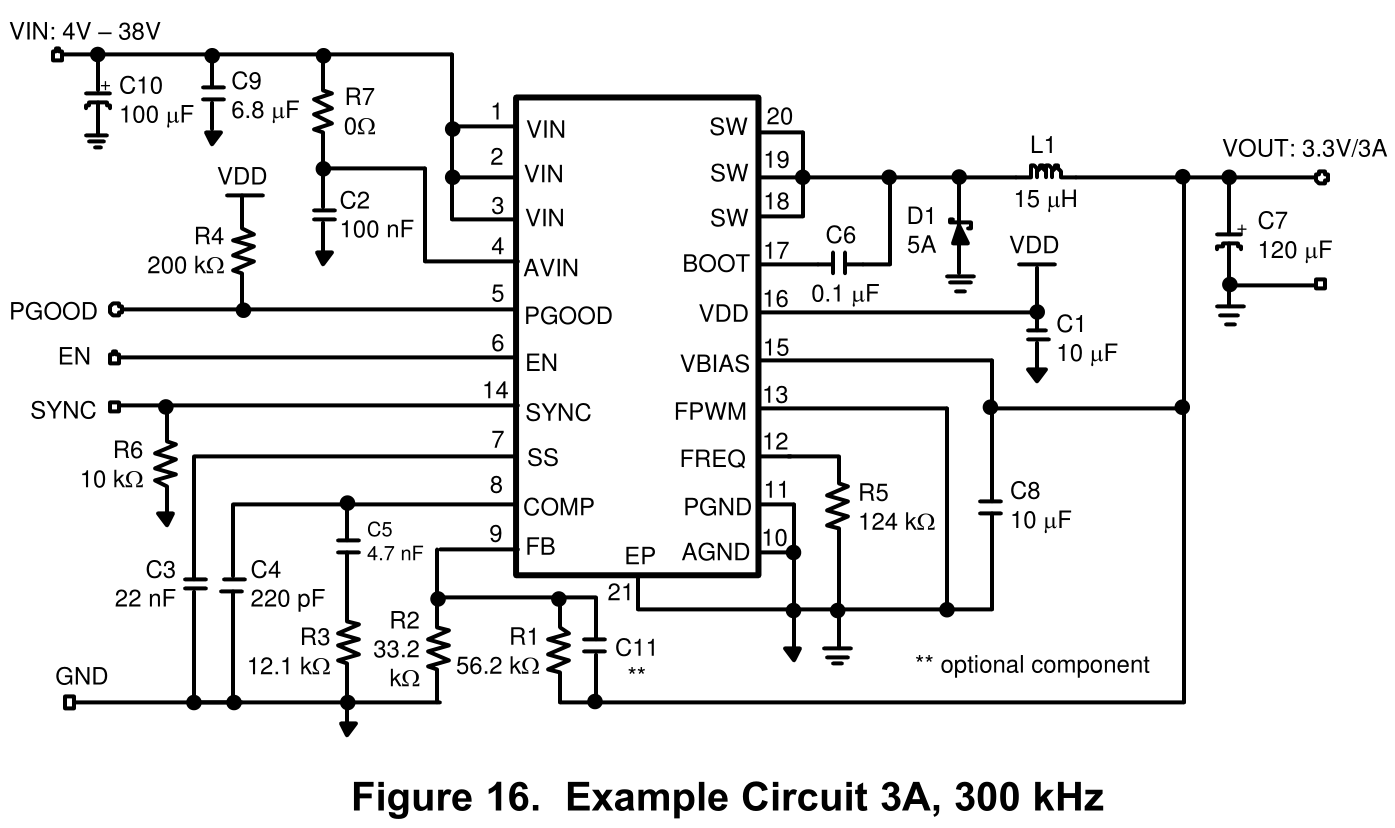
\includegraphics[width=\textwidth* 9/10]{../fig/billeder/lm26003fig16}
\label{fig:lm26003fig16}
\caption{Typisk kredsløb fra databladet for LM26003}
\end{figure}

Der er dog i forbindelse med udgangstrinnet lavet en modifikation ift. ''Typical Application'', som indebærer en 3V udgang. I forbindelse med L1 er der på samme kerne viklet viklinger på for at danne en transformer, hvorved en 3V udgang lavet. Denne rettes ud med en diode og en kondensator. 

